% Required packages: booktabs, graphicx, xcolor.
\newif\ifincludelegacy
\includelegacytrue
\newif\ifevalnotes
\evalnotestrue
\providecommand{\evalpending}[1]{\textcolor{blue!65!black}{[PENDING: #1]}}
\providecommand{\evalnote}[1]{\ifevalnotes\par\smallskip
  {\small\color{black!55}\noindent\textit{Draft note: #1}}\par\smallskip\fi}
\providecommand{\evalna}{\textcolor{blue!65!black}{--}}
\providecommand{\evalplot}[2]{%
  \IfFileExists{#1}{\includegraphics[width=\linewidth]{#1}}{%
    \fbox{\parbox[c][1.18in][c]{0.94\linewidth}{\centering\small
      \textbf{Figure layout --- measurements pending}\par\medskip #2}}}}


\section{Evaluation}
\label{sec:evaluation}

We evaluate \TITLE{} by asking four questions:
\begin{enumerate}
    \item How effectively does \TITLE{} serve concurrent zkML requests?
    \item How much does stage-aware admission improve resource utilization
          over whole-job peak reservation?
    \item Are historical stage profiles accurate enough for online admission?
    \item How much benefit comes from reusing setup artifacts?
\end{enumerate}

We additionally evaluate sensitivity to partition granularity and portability
to a second zkML backend.


\subsection{Experimental Setup}
\label{sec:eval-setup}



\textbf{Platforms.}
Single-node experiments run on a dual-socket AMD EPYC 9354 server with
64 physical cores and 128~GiB of RAM. Multi-node experiments use up to
10 AWS m6a.4xlarge instances, each with 16 vCPUs and 64~GiB of RAM.
One prover node also hosts the coordinator, and Amazon S3 is used for
artifact transfer between the coordinator and prover nodes.

\textbf{Workloads.}
We evaluate TinyBERT, MobileNetV2, and NanoGPT (4L), summarized in
Table~\ref{tab:models}. These workloads span transformer and convolutional
architectures and produce substantially different proof-job sizes and
resource demands. Unless otherwise stated, we use one ONNX operator per
partition. Section~\ref{sec:eval-granularity} evaluates sensitivity to
this choice.

\begin{table}[t]
\centering
% \small
\setlength{\tabcolsep}{3pt}
\renewcommand{\arraystretch}{1.18}
\begin{tabular}{@{}lccc@{}}
\toprule
Model & Input & Params (M) & Proof jobs \\
\midrule
TinyBERT       & Seq.\ 96              & 14.5 & 120 \\
MobileNetV2    & $3\times224\times224$ & 3.5  & 100 \\
NanoGPT (4L)   & Seq.\ 64              & 4.2  & 181 \\
\bottomrule
\end{tabular}
\caption{Primary evaluation workloads under the default partitioning
configuration.}
\label{tab:models}
\end{table}


% \begin{table}[t]
% \centering
% % \small
% \setlength{\tabcolsep}{3pt}
% \renewcommand{\arraystretch}{1.08}
% \begin{tabular*}{\columnwidth}{@{\extracolsep{\fill}}lrrrr@{}}
% \toprule
% & \multicolumn{2}{c}{Compute} & \multicolumn{2}{c}{Shared storage} \\
% \cmidrule(lr){2-3}\cmidrule(lr){4-5}
% Workload & Proving (s)   & Verify (s)  & S3 read (s) & S3 write (s) \\
%          % & (s)     & (s)    & (s)     & (s) \\
% \midrule
% NanoGPT (4L) & 746.3  & 7.1  & 264.0 & 20.3 \\
% MobileNetV2  & 4233.1 & 31.8 & 819.9 & 17.5 \\
% TinyBERT  & 4233.1 & 31.8 & 819.9 & 17.5 \\
% \bottomrule
% \end{tabular*}
% \caption{Mean aggregate job-level time across the 1--10 node
% scale-out runs. Execution and transfer times are summed across proof
% jobs and may overlap in wall-clock execution.}
% \label{tab:scaleout-overhead}
% \end{table}


\textbf{Policies.}
We compare three node-level execution policies while holding partitioning
and coordinator scheduling fixed. \emph{Fixed-$k$} limits each node to
\(k\) concurrently active proof jobs. \emph{Whole-job admission} reserves
each job's predicted peak memory until that job completes. \emph{\TITLE{}}
instead reserves the predicted memory of the execution stage about to run.
Unless otherwise stated, fixed concurrency uses \(k=8\); we evaluate
sensitivity to \(k\) separately.

\textbf{Profiles and setup.}
Cold runs generate setup artifacts during execution, while warm runs reuse
artifacts generated beforehand. Historical resource profiles are collected
in separate runs under the same setup condition and initialized identically
across compared policies.

\textbf{Traffic and metrics.}
Burst experiments submit \(N\in\{1,4,8,16\}\) requests simultaneously.
Sustained-load experiments use seeded Poisson arrivals so that all policies
receive the same request sequence. We report end-to-end request latency,
batch makespan, throughput, and peak memory, with additional runtime
measurements used to explain observed behavior.


\subsection{Performance Under Concurrent Requests}
\label{sec:eval-serving}

\begin{figure*}[t]
\centering
% \evalplot{figures/evaluation/burst_latency.pdf}{Three panels: MNIST GAN,
% MobileNetV2, NanoGPT. Horizontal axis: submitted requests (1, 4, 8, 16).
% Vertical axis: median request latency (minutes). Curves: selected Fixed-$k$,
% Whole-job, zkInfer. Warm setup; 256 GiB budget.}
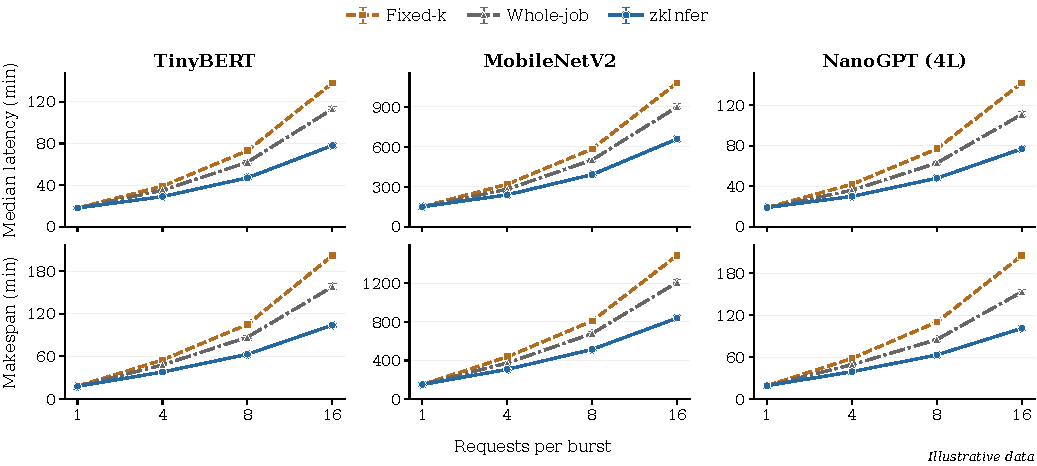
\includegraphics[width=0.95\linewidth]{figures/sacdad/eval/burst_serving.pdf}
\caption{End-to-end latency under burst arrivals on a single prover node.
We submit \(N\) inference requests simultaneously and compare fixed
concurrency, whole-job peak-memory admission, and \TITLE{}'s stage-aware
admission. Each panel shows one workload; lower is better.}
\label{fig:burst-performance}
\end{figure*}


We first examine how the three policies handle increasing
concurrent demand on a single prover node.
Figure~\ref{fig:burst-performance} reports mean request
completion time and burst makespan for each workload.


At \(N=1\), the comparison isolates concurrency among proof
jobs belonging to a single inference request.
\zkTBC{Describe the differences between policies and identify
which workloads benefit from overlapping jobs within a request.}
As \(N\) increases, jobs from multiple requests compete for
the same machine.
\zkTBC{Describe how completion time and makespan grow with
request count, including where the policies begin to diverge.}

At \(N=\zkTBC{N}\), stage-level admission changes mean request
completion time by \zkTBC{X\%} and makespan by \zkTBC{Y\%}
relative to whole-job reservation for \zkTBC{workload}.
\zkTBC{Explain whether the resource traces show additional
overlap during lower-memory stages, and report the associated
memory use and admission waiting.}
Compared with fixed concurrency, \zkTBC{describe whether
adaptive admission improves execution and where a fixed
limit remains competitive}.

The effect varies across workloads.
\zkTBC{Connect the observed differences to job heterogeneity,
stage-level memory variation, and CPU contention. Include
cases with little benefit or a regression.}
These results \zkTBC{state the supported conclusion about
stage-level admission under increasing concurrent demand}.


\subsection{Single-Request Scale-Out}
\label{sec:eval-scale-out}

We next examine how distributing proof jobs across machines affects the
completion time of an individual inference request. For each workload, we
hold the request and partitioning fixed and vary the prover pool from 1 to
10 nodes. Figure~\ref{fig:scale-out} reports request completion time and
speedup relative to one-node execution. Let \(T_p\) denote the completion
time using \(p\) prover nodes. We define speedup as \(T_1/T_p\).

All three workloads benefit substantially from additional nodes. NanoGPT
(4L) decreases from 1108~s on one node to 89~s on ten nodes, a
\(12.4\times\) speedup. MobileNetV2 decreases from 9639~s to 762~s,
yielding a \(12.7\times\) speedup, while TinyBERT decreases from 7900~s
to 750~s, a \(10.5\times\) speedup.
The scaling reflects effective distribution of the same proof workload
across additional nodes. At 10 nodes, summed job runtime per worker varies
by only 116.8--118.2~s for NanoGPT (4L) and 557.1--560.1~s for
MobileNetV2, while aggregate proving time remains nearly unchanged across
node counts. The reduction in completion time therefore comes primarily
from parallel execution rather than less proving work.

\textbf{Scale-out overhead.}
Table~\ref{tab:scaleout-overhead} breaks down aggregate job-level time
during the scale-out experiments. Proof generation remains the dominant
compute cost, averaging 746~s for NanoGPT (4L) and 4233~s for
MobileNetV2, compared with only 7~s and 32~s for verification. Shared
storage contributes mainly through reads rather than writes, with mean
aggregate S3 read times of 264~s and 820~s, while writes account for only
20~s and 18~s, respectively.
These transfer costs remain broadly stable as the prover pool grows.
Across 1--10 nodes, aggregate S3 read time ranges from 247--274~s for
NanoGPT and 798--848~s for MobileNetV2. Thus, increasing the number of
prover nodes does not substantially increase the total transfer cost for
a fixed request over the evaluated range, while proof generation remains
the dominant component.


% In the evaluation section
\begin{figure}[t]
    \centering
    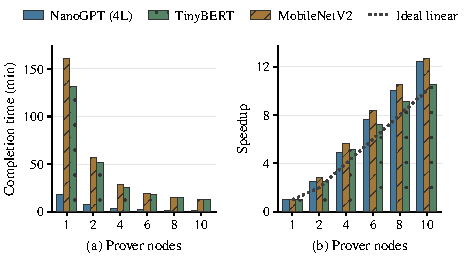
\includegraphics[width=\columnwidth]{figures/sacdad/eval/single_request_scaleout.pdf}
    \caption{
        Single-request scale-out across prover nodes.
        (a) Request completion time.
        (b) Speedup relative to one node, with ideal linear
        speedup shown as a dotted line.
        Partitioning and setup condition remain fixed.
    }
    \label{fig:scale-out}
\end{figure}

\begin{table}[t]
\centering
\small
\setlength{\tabcolsep}{3pt}
\renewcommand{\arraystretch}{1.08}
\begin{tabular*}{\columnwidth}{@{\extracolsep{\fill}}lrrrr@{}}
\toprule
& \multicolumn{2}{c}{Compute} & \multicolumn{2}{c}{Shared storage} \\
\cmidrule(lr){2-3}\cmidrule(lr){4-5}
Workload & Proving (s)   & Verify (s)  & S3 read (s) & S3 write (s) \\
         % & (s)     & (s)    & (s)     & (s) \\
\midrule
TinyBERT  & 4233.1 & 31.8 & 819.9 & 17.5 \\
MobileNetV2  & 4233.1 & 31.8 & 819.9 & 17.5 \\
NanoGPT (4L) & 746.3  & 7.1  & 264.0 & 20.3 \\


\bottomrule
\end{tabular*}
\caption{Mean aggregate job-level time across the 1--10 node
scale-out runs. Execution and transfer times are summed across proof
jobs and may overlap in wall-clock execution.}
\label{tab:scaleout-overhead}
\end{table}



% \subsection{Contribution of Resource-Management Mechanisms}
% \label{sec:eval-admission}

\subsection{Resource Profile Accuracy}
\label{sec:profile-accuracy}

\TITLE{} relies on recent executions of the same model partition to
estimate the memory required by each proving stage. We therefore evaluate
whether stage-level memory demand is sufficiently repeatable for this
history to support admission decisions. The microbenchmark repeatedly
executes representative partitions in isolation and records the peak
memory observed within each admission-relevant execution region. Cold
runs use the fused setup-and-prove region, while warm runs measure the
proving stage after reusable setup artifacts are available.

For each stage execution, we construct the prediction using only earlier
observations from the same partition and setup condition. With fewer than
five prior measurements, \TITLE{} uses the largest observed peak. Once
five observations are available, it uses the empirical 90th percentile
of the recent history. Figure~\ref{fig:profile-accuracy} reports the
median absolute prediction error and the fraction of predictions that
underestimate the subsequently observed peak.

Memory demand is highly repeatable across all three workloads. Median
absolute prediction error remains below 0.5\% in every measured
configuration. Under cold execution, the median error is 0.45\% for
MNIST GAN, 0.21\% for MobileNetV2, and 0.29\% for NanoGPT (4L). Warm
execution further reduces the error to 0.36\%, 0.15\%, and 0.07\%,
respectively. Some predictions still underestimate the observed peak, but the frequency
of these events should be interpreted together with their magnitude.
Underestimation occurs in 12.5--29.2\% of the measured cases, depending
on workload and setup condition. However, the resulting shortfalls are
small in the measurements available for these workloads, with the largest
observed shortfall remaining below 0.08~GiB. Thus, an underestimate
typically reflects a small deviation around an otherwise stable memory
profile rather than a large miss in required capacity.

\begin{figure}[t]
    \centering
    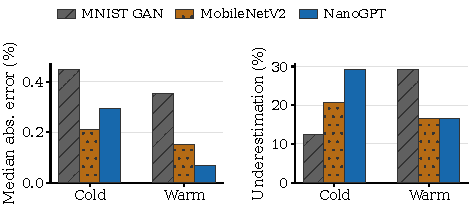
\includegraphics[width=\columnwidth]{figures/sacdad/eval/profile_accuracy_conditions.pdf}
    \caption{
    Accuracy of stage-level memory prediction under cold and warm
    execution. The left panel reports median absolute prediction error,
    while the right panel reports the fraction of predictions that
    underestimate observed memory demand. Predictions use only
    measurements from prior executions of the same partition and setup
    condition.
    }
    \label{fig:profile-accuracy}
\end{figure}

\subsection{Setup Reuse and Partition Granularity}
\label{sec:eval-sensitivity}

\textbf{Setup reuse.}
Table~\ref{tab:setup-reuse} compares the cost of generating
circuit-specific setup artifacts with reusing artifacts already available
in the node-local cache. Reuse reduces setup time by 98.6\% for TinyBERT,
97.3\% for MobileNetV2, and 96.3\% for NanoGPT (4L). In absolute terms,
MobileNetV2 falls from 14{,}609~s to 391~s, while TinyBERT and NanoGPT
fall from 1{,}636~s to 24~s and from 1{,}812~s to 67~s, respectively.
These reductions come with a sizeable storage footprint. The corresponding
proving keys occupy 68.8~GiB for TinyBERT, 287.5~GiB for MobileNetV2,
and 59.1~GiB for NanoGPT (4L). Reusing setup therefore removes most of
the repeated setup cost, but retaining every artifact locally is not
practical. This motivates the bounded per-node cache used by \TITLE{}.

\begin{table}[t]
\centering
\small
\setlength{\tabcolsep}{2.5pt}
\renewcommand{\arraystretch}{1.08}
\begin{tabular*}{\columnwidth}{@{\extracolsep{\fill}}lrrrr@{}}
\toprule
Workload & Gen. (s) & Reuse (s) & Saving (\%) & PK (GiB) \\
\midrule
TinyBERT      & 1{,}636.3  & 23.5  & 98.6 & 68.8 \\
MobileNetV2   & 14{,}608.7 & 391.0 & 97.3 & 287.5 \\
NanoGPT (4L)  & 1{,}812.3  & 67.1  & 96.3 & 59.1 \\
\bottomrule
\end{tabular*}
\caption{Cost of generating and reusing setup artifacts.}
\label{tab:setup-reuse}
\end{table}

\begin{figure}[t]
    \centering
    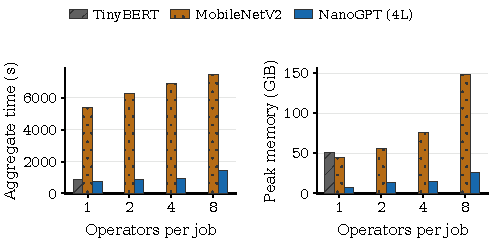
\includegraphics[width=\columnwidth]{figures/sacdad/eval/partition_granularity.pdf}
    \caption{
        Effect of partition granularity on proving cost and memory demand.
        Increasing the number of operators per proof job increases aggregate
        prover time and the peak memory required by individual jobs.
        }
\label{fig:partition-granularity}
    \label{fig:partition-granularity}
\end{figure}


\textbf{Partition granularity.}
We vary the number of operators grouped into each proof job while holding
the model and proving backend fixed. Figure~\ref{fig:partition-granularity}
shows that coarser partitions increase both aggregate prover time and peak
job memory, while exposing fewer independently schedulable jobs. We
therefore use one operator per proof job in the main serving experiments,
which provides the finest scheduling granularity and the lowest resource
demand among the configurations evaluated.


% \subsection{Contribution of Resource-Management Mechanisms}
% \label{sec:eval-admission}

% \paragraph{Memory reservation granularity.}
% To isolate admission, we compare whole-job and stage reservations while retaining
% the same coordinator policy, artifact state, and profile history. We repeat the
% eight- and sixteen-request experiments under 64, 128, and 256~GiB budgets.
% Figure~\ref{fig:eval-memory} reports the sixteen-request results. Each selected
% budget must accommodate the largest eligible job; an infeasible configuration is
% marked as such rather than treated as a completed run.

% \begin{figure*}[t]
% \centering
% \evalplot{figures/evaluation/memory_budget.pdf}{Two rows (cold, warm) by three
% workloads. Horizontal axis: usable memory budget (64, 128, 256 GiB).
% Vertical axis: batch makespan (minutes). Two curves: Whole-job and zkInfer.
% Sixteen requests per trial.}
% \caption{Effect of memory budget and reservation granularity on batch makespan.
% CPU capacity and coordinator policy remain fixed. Cold and warm executions use
% separate, matching histories. Error bars show the range across repeated trials.}
% \label{fig:eval-memory}
% \end{figure*}

% We compare the timing results with actual memory consumption and admission waits.
% A representative execution trace shows which stages overlap and whether the
% node remains memory-limited or instead reaches a CPU or storage bottleneck.
% Whole-job reservations cover the prover pipeline and output publication;
% supervisor-side artifact materialization precedes that reservation in the current
% implementation. The same boundary is used in every whole-job run. Keeping the
% selection policy fixed does not imply identical job order, since admission can
% change when jobs become runnable.
% \evalpending{Quantify improvements or regressions, peak actual memory, failures,
% and the cold/warm difference. Relate measured overlap to the motivation's packing
% opportunity without equating simulated makespan with real performance.}

% \paragraph{Coordinator scheduling.}
% We then keep stage admission enabled and compare request-fair FIFO, longest
% predicted job first within the selected request (LPT), and zkInfer's
% resource-aware coordinator policy. FIFO and LPT use the same current-free-memory
% feasibility check, so their comparison isolates within-request ordering more
% directly. The resource-aware policy additionally changes feasibility checking
% and uses cached setup and predicted duration as placement preferences. Its
% comparison is therefore a coordinator-policy ablation, not an isolated test of
% cache locality or LPT. Request fairness remains enabled in all three policies.

% \begin{table}[t]
% \centering\small\setlength{\tabcolsep}{3pt}
% \begin{tabular}{llrrr}
% \toprule
% Model & Policy & \shortstack{Median\\(min)} & \shortstack{Maximum\\(min)} & \shortstack{Failed\\requests}\\
% \midrule
% MNIST GAN & FIFO & \evalna & \evalna & \evalna\\
% & LPT & \evalna & \evalna & \evalna\\
% & zkInfer & \evalna & \evalna & \evalna\\
% MobileNetV2 & FIFO & \evalna & \evalna & \evalna\\
% & LPT & \evalna & \evalna & \evalna\\
% & zkInfer & \evalna & \evalna & \evalna\\
% NanoGPT & FIFO & \evalna & \evalna & \evalna\\
% & LPT & \evalna & \evalna & \evalna\\
% & zkInfer & \evalna & \evalna & \evalna\\
% \bottomrule
% \end{tabular}
% \caption{Coordinator-policy ablation with stage admission, warm setup,
% 16 requests, and a 256~GiB budget. Latency columns report means of per-trial
% statistics; failed requests are counted across trials. Dashes are pending.}
% \label{tab:eval-scheduling}
% \end{table}

% Table~\ref{tab:eval-scheduling} reports the resulting request latencies. For the
% mixed workload, we additionally normalize each request's latency by its model's
% isolated latency under the same setup condition. This avoids treating a naturally
% longer model as unfairly delayed solely because its absolute latency is larger.
% \evalpending{Explain which scheduling choices affect request completion and
% whether the benefit is consistent across models; report per-model slowdown for
% the mixture. A pure locality or fairness-off claim needs a separate toggle.}

% \paragraph{Setup reuse.}
% \label{sec:eval-reuse}

% The characterization established the aggregate setup time and storage associated
% with reusable artifacts. Here we measure the effect on complete requests,
% including queueing and concurrent execution. We compare cold and warm zkInfer
% runs for one and eight requests, holding partitioning, hardware, admission, and
% coordinator policy fixed. Each condition uses matching historical profiles.
% Cold runs regenerate setup; warm runs load matching artifacts from local files.

% \begin{table}[t]
% \centering\small\setlength{\tabcolsep}{3pt}
% \begin{tabular}{lrrrr}
% \toprule
% & \multicolumn{2}{c}{One request (min)} & \multicolumn{2}{c}{Eight requests (min)}\\
% \cmidrule(lr){2-3}\cmidrule(lr){4-5}
% Model & Cold & Warm & Cold & Warm\\
% \midrule
% MNIST GAN & \evalna & \evalna & \evalna & \evalna\\
% MobileNetV2 & \evalna & \evalna & \evalna & \evalna\\
% NanoGPT (4L) & \evalna & \evalna & \evalna & \evalna\\
% \bottomrule
% \end{tabular}
% \caption{Effect of setup reuse on completion time. One-request columns report
% request latency; eight-request columns report batch makespan. Entries are trial
% means; dashes mark pending measurements.}
% \label{tab:eval-reuse}
% \end{table} Table~\ref{tab:eval-reuse} connects avoided setup work to request-level benefit.
% Warm execution also changes which stages consume time and memory, so its effect
% on concurrency need not equal the reduction in summed setup time. We interpret
% the completion-time results together with setup-hit counts and measured loading
% costs. \evalpending{Report the observed latency/makespan reductions and explain
% any departure from the aggregate setup-time savings. Do not interpret these
% local-reuse measurements as a quantified remote-retrieval or locality benefit.}






% \subsection{Impact of Partition Granularity}
% \label{sec:eval-granularity}

% Partition granularity determines both the cost of individual
% proof jobs and the number of jobs available for concurrent
% execution. Combining more operators into each partition
% reduces the number of jobs, but may increase their execution
% time and memory requirements. We evaluate how this trade-off
% affects zkInfer's end-to-end performance.

% \textbf{Method.}
% For each of the three primary workloads, we vary the maximum
% number of operators per partition over
% $g \in \{1,2,4,8\}$. Operators are grouped consecutively in
% topological order, with $g=1$ corresponding to the default
% operator-level partitioning. All configurations use zkInfer's
% stage-based admission, the same prover thread settings, and
% a 256~GiB proof-memory budget on the single-node platform.
% We collect separate resource profiles and generate matching
% setup artifacts for each partitioning configuration.

% We evaluate a single inference request and a fixed batch of
% sixteen simultaneously submitted requests. The single-request
% experiment measures how granularity affects the completion
% of one inference, while the batch experiment examines how
% the resulting jobs share resources across requests.
% We report single-request latency and batch makespan across
% three trials per configuration. The $g=1$ results are reused
% from Section~\ref{sec:eval-serving}.

% \begin{figure*}[t]
% \centering
% \evalplot{figures/evaluation/partition_granularity.pdf}{
% Two rows by three workload columns: MNIST GAN,
% MobileNetV2, and NanoGPT (4L).
% Horizontal axis: maximum operators per partition,
% $g \in \{1,2,4,8\}$.
% Top row: single-request latency (minutes).
% Bottom row: sixteen-request batch makespan (minutes).
% One curve per panel: zkInfer.
% Points show the median across three trials;
% error bars show the observed minimum and maximum.
% }
% \caption{Sensitivity of zkInfer to partition granularity
% under a 256~GiB proof-memory budget.
% Each column corresponds to one workload.
% Setup artifacts are reused, and each partitioning
% configuration uses matching resource profiles.
% Lower completion times are better.}
% \label{fig:eval-granularity}
% \end{figure*}

% \textbf{Single-request performance.}
% Figure~\ref{fig:eval-granularity} shows how request latency
% changes as more operators are assigned to each proof job.
% \evalpending{Report the latency at each granularity, identify
% the best observed configuration for each workload, and
% quantify the difference relative to $g=1$. State whether
% the trend is monotonic or whether an intermediate
% granularity performs best.}

% To interpret these results, we examine the isolated job
% profiles collected for each configuration. Aggregate job
% duration captures changes in total execution work, while
% the longest job and largest memory footprint indicate
% potential limits on concurrent execution.
% \evalpending{Connect the observed latency changes to measured
% changes in these quantities and to runtime admission waiting.
% Do not attribute an improvement to lower scheduling or
% communication overhead unless the corresponding measurements
% support that explanation.}

% \textbf{Concurrent-request performance.}
% The sixteen-request experiment holds the total number of
% inferences fixed while changing the proof jobs generated
% by each request.
% \evalpending{Report batch makespan across granularities and
% the change relative to $g=1$. Explain whether the preferred
% granularity matches the single-request result, and whether
% the performance differences become larger or smaller under
% concurrent requests.}

% Multiple requests provide additional independent jobs that
% may compensate for the reduced job count of a coarser
% partitioning. However, larger per-job memory requirements
% can still restrict how many jobs execute together.
% \evalpending{Use measured memory demand, admission waiting,
% and worker utilization to explain which effect is visible
% in the results. If the measurements do not distinguish the
% causes, describe the observed trend without assigning one.}

% \textbf{Implication.}
% \evalpending{State whether the default $g=1$ configuration
% performs best, remains close to the best observed result,
% or incurs a meaningful penalty. Quantify that conclusion
% and identify any workload-dependent exceptions. If a coarser
% configuration performs better, distinguish the default's
% simplicity from its measured performance rather than
% claiming that operator-level partitioning is optimal.}

